\documentclass[a4paper]{article}
\usepackage[utf8]{inputenc}


%=-=-=-=-=-=-=-=-=-=-=-=-=-=-=-=-=-=-=-=-=-=-=-=-=-=-=-=-=-=-=-=-=-=-=-=-=-=-=-=-
% PREAMBLE
%=-=-=-=-=-=-=-=-=-=-=-=-=-=-=-=-=-=-=-=-=-=-=-=-=-=-=-=-=-=-=-=-=-=-=-=-=-=-=-=-

%%%%%%%%%%%%%%%%%%%%%%%%%%%%%%%%%%%%%%%%%%%%%%%%%%%%%%%%%%%%%%%%%%%%%
% Important styling notes
%%
% For now, to include img.jpg in img/path/to/img.jpg, just use:
% path/to/img.jpg - for details see style.tex
%=-=-=-=-=-=-=-=-=-=-=-=-=-=-=-=-=-=-=-=-=-=-=-=-=-=-=-=-=-=-=-=-=-=-=-=-=-=-=-=-
% Packages
%%
%\usepackage{fullpage} % Package to use full page
\usepackage[top=1in,bottom=1in,left=1in,right=0.7in,heightrounded]{geometry}

\usepackage{parskip}                    % Package to tweak paragraph skipping
\usepackage{amsmath}                    % standard
\usepackage{amssymb}                    % standard - Double R symbol etc.
\usepackage{hyperref}
\usepackage{amsthm}                     % standard - theorem, definition, etc.
\usepackage{multicol}                   % multiple columns for numbering
\usepackage{enumitem}                   % standard - enumerate styles
\usepackage[utf8]{inputenc}
\usepackage{scrextend}                  % indentation
\usepackage{graphicx}                   % standard - add figures
\usepackage{float}                      % standard - figure position, use [H] option
\usepackage{pifont}                     % symbols
\usepackage{gensymb}                    % degree symbol \degree
\usepackage{xcolor}                     % bg color
\hypersetup{
    colorlinks,
    linkcolor={black!50!black},
    citecolor={blue!50!black},
    urlcolor={blue!80!black}
}
\usepackage{framed}                     % bg color
\usepackage[T1]{fontenc}                % small caps
\usepackage{sectsty}                    % headings colour
\usepackage{mathtools}                  % Loads amsmath
\usepackage{amsthm,thmtools,xcolor}     % coloured theorem
\usepackage[toc,page]{appendix}         % reference to appendix
%\usepackage{titlesec}                   % change chapter, section, etc. formats
\usepackage{xifthen}                    % if, else
\usepackage{etoolbox}
% format numbering in theorem, lemma, etc. environment
\AtBeginEnvironment{theorem}{\setlist[enumerate, 1]{font=\upshape,  wide=0.5em, before=\leavevmode}}
\AtBeginEnvironment{lemma}{\setlist[enumerate, 1]{font=\upshape,  wide=0.5em, before=\leavevmode}}
\usepackage[letterspace=150]{microtype} % \textls{<letterspaced text>} % 0 <= letterspace <= 1000, 1000 = M space
\usepackage{letltxmacro}                % renew commands?
\usepackage{minted}                     % package to list code
    % otherwise minted goes off the page
    \setmintedinline{breaklines}
\usepackage{subfig}
\usepackage{eso-pic}                    % title page bg pic
\usepackage{varwidth}
\PassOptionsToPackage{svgnames}{xcolor}
\usepackage{fontawesome}                % \faQuestionCircle
\usepackage{marvosym}                   %\Pointinghand
\usepackage{mdframed}                   % easy outline frames
\usepackage[many]{tcolorbox}            % colour box for theorem styles
\usepackage{array,booktabs,calc} % table figs and text
\usepackage{comment}                    % \begin{comment}
\usepackage{fancyhdr}                   % page headings
\usepackage{mdframed}                   % boxes
\usepackage[backend=biber,sorting=none,style=ieee]{biblatex}
\usepackage{caption}
%%% caption options {
%\DeclareCaptionFont{white}{\color{white}}
\DeclareCaptionFormat{listing}{\colorbox{magenta!30!gray}{\parbox{\textwidth}{#1#2#3}}}
\captionsetup[lstlisting]{format=listing,labelfont={bf,small},textfont=small,skip=-1pt}
%%% }
\addbibresource{bibliography.bib}
\usepackage{url}
\usepackage{textcomp}
\usepackage[makeroom]{cancel}            % crossed symbols
\usepackage{algorithm}
\usepackage[noend]{algpseudocode}
\usepackage{tikz}
\usetikzlibrary{arrows.meta,positioning,quotes} % arrows and nodes in tikz
\usepackage{marginnote}
\usepackage{pgfplots}
\usepackage{pstricks-add,pst-slpe}  % for fancy tikz arrows
%\usepackage{titlesec}                   % title style
\usepackage{lmodern}                    % a font
\usepackage{titletoc} % Required for manipulating the table of contents
\usepackage{titlesec} % Allows customization of titles
\usepackage{fouriernc} % Use the New Century Schoolbook font
\usepackage{booktabs} % things in page margins
\usepackage{stmaryrd } % \varoast
\usepackage{listings} % code listings
\usepackage{longtable} % table across multiple pages
\usepackage{styles/nasm/lang}  % include custom language for NASM assembly.
\usepackage{styles/nasm/style} % include custom style for NASM assembly.



%% extra comments that I don't know where they belong:
% list of ding tags: http://willbenton.com/wb-images/pifont.pdf

%=-=-=-=-=-=-=-=-=-=-=-=-=-=-=-=-=-=-=-=-=-=-=-=-=-=-=-=-=-=-=-=-=-=-=-=-=-=-=-=-
% Colours for various things
%%


\definecolor{shadecolor}{rgb}{1.,0.933,0.96} % bg color, r,g,b <= 1
\definecolor{medium_blue}{RGB}{60,125,190}
\definecolor{dark_blue}{RGB}{25,60,85}
\definecolor{dark_red}{RGB}{77,16,16}
\definecolor{LightPink}{rgb}{0.92.,0.8,0.84} % bg color, r,g,b <= 1
\definecolor{LighterPink}{rgb}{1.,0.94,0.97} % bg color, r,g,b <= 1
\definecolor{LightestPink}{rgb}{1.,0.95,0.99} % bg color, r,g,b <= 1
\definecolor{DarkestPink}{rgb}{0.36, 0.0, 0.18}
\definecolor{DarkerPink}{rgb}{0.41, 0.0, 0.21}
\definecolor{DarkPink}{rgb}{0.55, 0.05, 0.37}
\definecolor{lightestestpink}{RGB}{255,248,252}
\definecolor{codegray}{rgb}{0.5,0.5,0.5}
\definecolor{codegrayblue}{rgb}{0.35,0.35,0.47}



%=-=-=-=-=-=-=-=-=-=-=-=-=-=-=-=-=-=-=-=-=-=-=-=-=-=-=-=-=-=-=-=-=-=-=-=-=-=-=-=-
% Define my own theorem styles
%%

% "base" styles
\declaretheoremstyle[
  headfont=\color{DarkPink}\bfseries,
  bodyfont=\itshape,
]{colored}

\declaretheoremstyle[
  headfont=\color{DarkPink}\bfseries,
  bodyfont=\normalfont,
]{colored_upright}

% theorems (corollaries, etc) themselves, inherit from my style above
% Usage:
% \begin{theorem} \end{theorem}, \begin{lemma} \end{lemma}, ...
\declaretheorem[
	numberwithin=section,
 	style=colored,
	name=\textsc{Theorem},
]{theorem}

\tcolorboxenvironment{theorem}{
  boxrule=0pt,
  boxsep=2pt,
  colback={magenta!25!white},
  colframe=DarkPink,
  enhanced jigsaw, 
  borderline west={2pt}{0pt}{DarkPink},
  sharp corners,
  before skip=5pt,
  after skip=5pt,
  breakable,
  right=0mm % for equations
}

\declaretheorem[
	numberwithin=section,
 	style=colored,
	name=\textsc{Corollary},
]{corollary}

\tcolorboxenvironment{corollary}{
  boxrule=0pt,
  boxsep=1pt,
  colback={magenta!10!white},
  colframe=DarkPink,
  enhanced jigsaw, 
  borderline west={2pt}{0pt}{DarkPink},
  sharp corners,
  before skip=5pt,
  after skip=5pt,
  breakable,
  right=0mm % for equations
}

\declaretheorem[
	numberwithin=section,
	style=colored,
	name=\textsc{Lemma},
]{lemma}

\tcolorboxenvironment{lemma}{
  boxrule=0pt,
  boxsep=1pt,
  colback={magenta!10!white},
  colframe=DarkPink,
  enhanced jigsaw, 
  borderline west={2pt}{0pt}{DarkPink},
  sharp corners,
  before skip=5pt,
  after skip=5pt,
  breakable,
  right=0mm % for equations
}

\declaretheorem[
	numberwithin=section,
	style=colored,
	name=\textsc{Definition},
]{definition}

\tcolorboxenvironment{definition}{
  boxrule=0pt,
  boxsep=1pt,
  colback={magenta!25!white},
  colframe=DarkPink,
  enhanced jigsaw, 
  borderline west={2pt}{0pt}{DarkPink},
  sharp corners,
  before skip=5pt,
  after skip=5pt,
  breakable,
  right=0mm % for equations
}

\declaretheorem[
	numberwithin=section,
  	style=colored,
  	name=\textsc{Example},
]{exmp}

\declaretheorem[
	numberwithin=section,
  	style=colored,
  	name=\textsc{Solution},
]{soln}

%%% code listings
\lstdefinestyle{code1}{
    backgroundcolor=\color{lightestestpink},   
    commentstyle=\color{codegrayblue},
    keywordstyle=\color{DarkerPink},
    numberstyle=\tiny\color{codegray},
    stringstyle=\color{black!40!cyan},
    basicstyle=\small\ttfamily,
    breakatwhitespace=false,
    breaklines=true,        
    captionpos=t,             
    keepspaces=true,        
    numbers=left,           
    numbersep=5pt,
    showspaces=false, 
    showstringspaces=false,
    showtabs=false,
    tabsize=4
}

\lstset{style=code1}

%=-=-=-=-=-=-=-=-=-=-=-=-=-=-=-=-=-=-=-=-=-=-=-=-=-=-=-=-=-=-=-=-=-=-=-=-=-=-=-=-
% Headers (size, font, colour)
%%




\makeatletter
\renewcommand{\@seccntformat}[1]{\llap{\textcolor{DarkestPink}{\csname the#1\endcsname}\hspace{1em}}}                    
\renewcommand{\section}{\@startsection{section}{1}{\z@}
{-4ex \@plus -1ex \@minus -.4ex}
{1ex \@plus.2ex }
{\normalfont\large\sffamily\bfseries\textcolor{DarkestPink}}}
\renewcommand{\subsection}{\@startsection {subsection}{2}{\z@}
{-3ex \@plus -0.1ex \@minus -.4ex}
{0.5ex \@plus.2ex }
{\normalfont\sffamily\bfseries\textcolor{DarkestPink}}}
\renewcommand{\subsubsection}{\@startsection {subsubsection}{3}{\z@}
{-2ex \@plus -0.1ex \@minus -.2ex}
{.2ex \@plus.2ex }
{\normalfont\small\sffamily\bfseries\textcolor{DarkestPink}}}                        


%=-=-=-=-=-=-=-=-=-=-=-=-=-=-=-=-=-=-=-=-=-=-=-=-=-=-=-=-=-=-=-=-=-=-=-=-=-=-=-=-
% Numberings, counters and spacings
%%
\numberwithin{equation}{section} % section number in eq/s
\setlength{\jot}{7pt} % spacing in split, gathered env/s



%% Custom examples
%% Output - Example 1,2,...
\newcounter{example}
\newenvironment{example}[1][]{\refstepcounter{example}\par\medskip
   \textbf{Example~\theexample. #1} \rmfamily}{\medskip}
%%%%%%%%%%%% End of unused %%%%%%%%%%%%



%=-=-=-=-=-=-=-=-=-=-=-=-=-=-=-=-=-=-=-=-=-=-=-=-=-=-=-=-=-=-=-=-=-=-=-=-=-=-=-=-
% Paths
%%
\graphicspath{ {./img/} } % figures' path - can look up files directly from there


%=-=-=-=-=-=-=-=-=-=-=-=-=-=-=-=-=-=-=-=-=-=-=-=-=-=-=-=-=-=-=-=-=-=-=-=-=-=-=-=-
% User defined macros (math mode)
%%


% Curly braces under text. Usage: \myunderbrace{upper}{lower}
\newcommand{\myunderbrace}[2]{\mathrlap{\underbrace{\phantom{#1}}_{#2}} #1}
\newcommand{\setR}{\mathbb{R}} % \ouble R
\newcommand{\setRn}{\mathbb{R}^n} %  double R^n
\newcommand{\setN}{\mathbb{N}} % double N
\newcommand{\setZ}{\mathbb{Z}} % double Z
\let\oldemptyset\emptyset
\let\emptyset\varnothing % nice - looking empty set symbol
\newcommand{\fancyN}{\mathcal{N}} % null space
\newcommand{\fancyR}{\mathcal{R}} % range

\newcommand{\bx}{\textbf{x}}
\newcommand{\by}{\textbf{y}}
\newcommand{\bb}{\textbf{b}}
\newcommand{\bA}{\textbf{A}}
\newcommand{\bB}{\textbf{B}}
\newcommand{\bI}{\textbf{I}}
% double bars as in norm
\newcommand{\norm}[1] {\lVert #1 \rVert} 
\newcommand{\trans}[1]{#1^{\top}}

\newcommand{\mean}[1]{\bar{#1}}
\newcommand{\var}{\sigma^2}

\newcommand{\partdevx}[1]{\frac{\partial #1}{\partial x}}
\newcommand{\partdevxx}[1]{\frac{\partial #1}{\partial x}}
\newcommand{\partdevxn}[1]{\frac{\partial^n #1}{\partial x^n}}
\newcommand{\partdevy}[1]{\frac{\partial #1}{\partial x}}
\newcommand{\partdevyy}[1]{\frac{\partial #1}{\partial y}}
\newcommand{\partdevyn}[1]{\frac{\partial^n #1}{\partial y^n}}

% text above = symbol
\newcommand{\overeq}[1]{\ensuremath{\stackrel{#1}=}} 
\newcommand{\greatersmaller}{%
  \mathrel{\ooalign{\raisebox{.6ex}{$>$}\cr\raisebox{-.6ex}{$<$}}}
} % greater and smaller symbols on top of each other, same line

%=-=-=-=-=-=-=-=-=-=-=-=-=-=-=-=-=-=-=-=-=-=-=-=-=-=-=-=-=-=-=-=-=-=-=-=-=-=-=-=-
% User defined macros (non math)

\newcommand{\qedblack}{$\hfill\blacksquare$} % black square end of line
\newcommand{\qedwhite}{\hfill \ensuremath{\Box}} % white square end of line
\newcommand{\hquad}{\hskip0.5em\relax}% half quad space
%\newcommand{\TODO}{\textcolor{red}{\bf TODO!}\;}

\newcommand{\TODO}[1][]{%
    \ifthenelse{\equal{#1}{}}{\textcolor{red}{\bf TODO!}\;}{\textcolor{red}{\textbf {TODO:} #1}\; }%
}
\newcommand{\B}[1]{\textbf{\textup{#1}}} % bold and upright
\renewcommand{\labelitemi}{\scriptsize$\textcolor{DarkPink}{\blacksquare}$} % itemize - squares instead of bullets
\newcommand{\emphasis}[1]{\textls{#1}}

\LetLtxMacro{\originaleqref}{\eqref}
\renewcommand{\eqref}{Eq.~\originaleqref}
\renewcommand*{\eqref}[1]{Eq.~\originaleqref{#1}}





% background images
%%%%%%%
\newcommand\BackgroundPic{%
\put(0,0){%
\parbox[b][\paperheight]{\paperwidth}{%
\vfill
%\centering

\includegraphics[width=0.125\paperwidth,height=\paperheight,%
]{img/background_02.png}% use ,keepaspectratio
\vfill
}}}
%%%%%%%
% end of background image
%%%%%%%%%%%%%% my own frame
\newmdenv[topline=false,bottomline=false]{leftrightbox}
%%%%%%%%%%%%% end
%%%%%%%%%%%%% my own comment
\newcommand{\mycomment}[1]{\begin{leftrightbox}\Pointinghand~\textbf{Comment:}~#1 \end{leftrightbox}}
%%%%%%%%%%%%% end
% my custom note https://tex.stackexchange.com/questions/301993/create-custom-note-environment-with-tcolorbox
\newmdenv[
    topline=false,
    bottomline=false,
    rightline=false,
    innerrightmargin=0pt
]{siderule}
\newenvironment{mynote}%
    {\begin{siderule}\textbf{\Pointinghand~Note:}}
    {\end{siderule}}
%%%%%%%%%%%%% my own box
\newcommand{\boxone}[1]{\begin{tcolorbox}[colback = LighterPink,colframe=LightPink]
#1
\end{tcolorbox}}
%%%%%%%%%%%%% end

\let\oldemptyset\emptyset
\let\emptyset\varnothing
%algorithmic
\algdef{SE}[DOWHILE]{Do}{doWhile}{\algorithmicdo}[1]{\algorithmicwhile\ #1}%






\begin{document}
%=-=-=-=-=-=-=-=-=-=-=-=-=-=-=-=-=-=-=-=-=-=-=-=-=-=-=-=-=-=-=-=-=-=-=-=-=-=-=-=-
% GLOBAL STYLES (DOCUMENT SCOPE)
%=-=-=-=-=-=-=-=-=-=-=-=-=-=-=-=-=-=-=-=-=-=-=-=-=-=-=-=-=-=-=-=-=-=-=-=-=-=-=-=-
% caption: Figure 1 -> <bold> Fig. 1 </bold>
\captionsetup[figure]{labelfont={bf},labelformat={default},labelsep=period,name={Fig.}}


%=-=-=-=-=-=-=-=-=-=-=-=-=-=-=-=-=-=-=-=-=-=-=-=-=-=-=-=-=-=-=-=-=-=-=-=-=-=-=-=-
% TITLE PAGE
%=-=-=-=-=-=-=-=-=-=-=-=-=-=-=-=-=-=-=-=-=-=-=-=-=-=-=-=-=-=-=-=-=-=-=-=-=-=-=-=-
%%%%%%%%%%%%%%%%%%%%%%%%%%%%%%%%%%%%%%%%%
% Formal Book Title Page
% LaTeX Template
% Version 2.0 (23/7/17)
%
% This template was downloaded from:
% http://www.LaTeXTemplates.com
%
% Original author:
% Peter Wilson (herries.press@earthlink.net) with modifications by:
% Vel (vel@latextemplates.com)
%
% License:
% CC BY-NC-SA 3.0 (http://creativecommons.org/licenses/by-nc-sa/3.0/)
% 
% This template can be used in one of two ways:
%
% 1) Content can be added at the end of this file just before the \end{document}
% to use this title page as the starting point for your document.
%
% 2) Alternatively, if you already have a document which you wish to add this
% title page to, copy everything between the \begin{document} and
% \end{document} and paste it where you would like the title page in your
% document. You will then need to insert the packages and document 
% configurations into your document carefully making sure you are not loading
% the same package twice and that there are no clashes.
%
%%%%%%%%%%%%%%%%%%%%%%%%%%%%%%%%%%%%%%%%%

%----------------------------------------------------------------------------------------
%	PACKAGES AND OTHER DOCUMENT CONFIGURATIONS
%----------------------------------------------------------------------------------------



%----------------------------------------------------------------------------------------
%	TITLE PAGE
%----------------------------------------------------------------------------------------



\begin{titlepage} % Suppresses headers and footers on the title page

	\centering % Centre everything on the title page
	
	\scshape % Use small caps for all text on the title page
	
	\vspace*{\baselineskip} % White space at the top of the page
	
	%------------------------------------------------
	%	Title
	%------------------------------------------------
	
	\rule{\textwidth}{1.6pt}\vspace*{-\baselineskip}\vspace*{2pt} % Thick horizontal rule
	\rule{\textwidth}{0.4pt} % Thin horizontal rule
	
	\vspace{0.75\baselineskip} % Whitespace above the title
	
	{\LARGE COMPUTER VISION NOTES\\ \Large OBJECT LOCALISATION AND TRACKING\\} % Title
	
	\vspace{0.75\baselineskip} % Whitespace below the title
	
	\rule{\textwidth}{0.4pt}\vspace*{-\baselineskip}\vspace{3.2pt} % Thin horizontal rule
	\rule{\textwidth}{1.6pt} % Thick horizontal rule
	
	\vspace{2\baselineskip} % Whitespace after the title block
	
	%------------------------------------------------
	%	Subtitle
	%------------------------------------------------
	My personal notes on
	
	\vspace*{3\baselineskip} % Whitespace under the subtitle
	
	Object Localisation Techniques; Colour Matching, Mean Shift Tracking, Optical Flow, Lukas Kanade 
	
	\vspace*{3\baselineskip} % Whitespace under the subtitle
	
	%------------------------------------------------
	%	Editor(s)
	%------------------------------------------------
	
	By
	
	\vspace{0.5\baselineskip} % Whitespace before the editors
	
	{\normalfont \Large \mintinline{latex}{0xLeo} (\url{github.com/0xleo}) \\} % Editor list
	
	\vspace{0.5\baselineskip} % Whitespace below the editor list
	
	%\textit{The University of California \\ Berkeley} % Editor affiliation
	
	\vfill % Whitespace between editor names and publisher logo
	
	%------------------------------------------------
	%	Publisher
	%------------------------------------------------
	
	
	\vspace{0.3\baselineskip} % Whitespace under the publisher logo
	
	\today % Date
	
	{DRAFT X.YY} % Draft version
	{\\Missing: \ldots}

\end{titlepage}

%----------------------------------------------------------------------------------------

%\maketitle



%=-=-=-=-=-=-=-=-=-=-=-=-=-=-=-=-=-=-=-=-=-=-=-=-=-=-=-=-=-=-=-=-=-=-=-=-=-=-=-=-
% MAIN DOCUMENT
%=-=-=-=-=-=-=-=-=-=-=-=-=-=-=-=-=-=-=-=-=-=-=-=-=-=-=-=-=-=-=-=-=-=-=-=-=-=-=-=-
\newpage
\tableofcontents
\newpage



%------------------------------ New section ------------------------------%
\section{Projective geometry}


\subsection{Homogeneous coordinates}


\subsubsection{Motivation}
Homogeneous coordinates (H.C.) are a way of representing points and lines. In the homogeneous space, it is easier to formalise some mathematical derivations than in the Euclidean space. Homogeneous coordinates are often used in computer vision mainly in two broad applications.
\begin{enumerate}
    \item They allow us to \textit{compactly represent point transforms}. For instance, they allow us to represent the affine transform (rotation and translation) as a matrix multiplication $\by = \bA\bx$ as opposed to $\by = \textbf{R}\bx + \textbf{T}$, where $\bA$ (affine matrix) embeds $\textbf{R}$ (rotation) and $\textbf{T}$ (translation). To see why this is the case, consider the rotation and translation mapping of a point $\begin{bmatrix}x_1 & x_2 & x_3\end{bmatrix}\t$ given by:
    % ref https://math.stackexchange.com/questions/1155986/why-use-homogeneous-coordinates
    \[
        \begin{bmatrix} x_1 \\ x_2 \\ x_3 \end{bmatrix} \mapsto
        \underbrace{
            \begin{bmatrix}
            r_{11} & r_{12} & r_{13} \\
            r_{21} & r_{22} & r_{23} \\
            r_{31} & r_{32} & r_{33} \\
            \end{bmatrix}
        }
        _{\textbf{R}}
        \underbrace{\begin{bmatrix} x_1 \\ x_2 \\ x_3 \end{bmatrix} +}_{\bx}
        \underbrace{\begin{bmatrix} t_1 \\ t_2 \\ t_3 \end{bmatrix}}_{\textbf{T}}
    \]
    This can be written as a single matrix multiplication, which is more compact and also allows computer programs to optimise it.
    
    The trick is to pack \textbf{}$\textbf{R}$ and $\textbf{T}$ into one $3\times 4$ matrix $\begin{bmatrix}
    \textbf{R} \; | \; \textbf{T}
    \end{bmatrix}$ by appending $\textbf{T}$ to $\textbf{R}$:
    \[
    \begin{bmatrix}
    \textbf{R}\; | \; \textbf{T}
    \end{bmatrix} = 
    \begin{bmatrix}
        r_{11} & r_{12} & r_{13} & t_1 \\
        r_{21} & r_{22} & r_{23} & t_2 \\
        r_{31} & r_{32} & r_{33} & t_3 \\
    \end{bmatrix}
    \]
    \marginnote{We can convert a Euclidean point to hom. by appending a new extra coordinate with value 1.}This is the so-called \emphasis{affine} matrix $\textbf{A}$. However, the multiplication of $\bA$ with $\bx$ is undefined as $\bx$ is $3 \times 1$. The can augment $\bx$ to the size $4 \times 1$ by introducing a new (redundant) coordinate $x_4=1$. But now the product $\begin{bmatrix}\textbf{R}\; | \; \textbf{T}\end{bmatrix} \bx$ is of size $3 \times 1$, which certainly does not belong in the homogeneous space of the original vector of length 4. So to keep $\begin{bmatrix}\textbf{R}\; | \; \textbf{T}\end{bmatrix} \bx$  an inner operation and to satisfy $\bx_{hom} = \bI_{hom}\bx_{hom}$  we add a fourth redundant row $\begin{bmatrix} 0 & 0 & 0 & 1\end{bmatrix}$. The final matrix
    \[
    \bA =     \begin{bmatrix}
        r_{11} & r_{12} & r_{13} & t_1 \\
        r_{21} & r_{22} & r_{23} & t_2 \\
        r_{31} & r_{32} & r_{33} & t_3 \\
        0 & 0 & 0 & 1
    \end{bmatrix}
    \]
    is an \emphasis{affine} matrix. $\begin{bmatrix} x_1 & x_2 & x_3 & 1 \end{bmatrix}$ is the H.C. form the Euclidean point $\begin{bmatrix} x_1 & x_2 & x_3\end{bmatrix}$. Using the affine matrix, translation can also be expressed as part of a matrix product.
    \[
    \by = \bA\bx = 
    \begin{bmatrix}
        \begin{matrix}
            \textbf{\large{R}} \quad |  \quad \textbf{\large{T}}
        \end{matrix} \\
        \begin{matrix}
            0 & 0 & 0 & 1
        \end{matrix}
    \end{bmatrix} \bx
    \]
    
    \item They can \textit{represent points at the projective plane}, i.e. 3D points from the ``real world'' mapped into a 2D plane (screen). They can even represent points at infinity via finite scalars; without running into divisions by zero. Projections ubiquitously take place in camera models, the simplest one being a \emphasis{pinhole camera}.
    
    Camera models, such as the pinhole map a 3D point $(x,y,z)$ in the ``real world'' onto a 2D plane (camera film/screen) using linear transforms. The linear transform depends on the internal manufacturing characteristics (a.k.a. \emphasis{intrinsics}) of the camera and the externals (\emphasis{extrinsics}), such as its translation and rotation. For the pinhole model, the only intrinsic we consider is the focal length $f$\footnote{The projected coordinates are in distance units for simplicity, so that we can stick to one instrinsic -- the focal length. If they were measured in pixels, we would include two more intrinsic parameters in the matrix.}. It can be easily derived (see \ref{app:pinhole_model_deriv}) that the pinhole camera projection is described by the following transform.
    \begin{equation}
        \begin{bmatrix}
            x\prime \\
            y\prime 
        \end{bmatrix} 
        =
        \begin{bmatrix}
            \frac{fx}{z} \\
            \frac{fy}{z} 
        \end{bmatrix} = 
         \frac{1}{z}\begin{bmatrix}
            f & 0 & 0 \\
            0 & f & 0 \\
            0 & 0 & 1
        \end{bmatrix}
        \begin{bmatrix}
            x \\ y \\ z
        \end{bmatrix}
        \label{eq:pinhole_model}
    \end{equation}
    H.C. allow us to express \eqref{eq:pinhole_model} as a linear transform, hence more concisely. Although \eqref{eq:pinhole_model} is simple, camera models can get complicated.
\end{enumerate}

% src https://math.stackexchange.com/a/1156000
Apart from points, H.C. also represent lines (via their coefficients). Lines appear virtually everywhere in images (e.g. edges). Homogeneous coordinates help us answer questions about the correspondences of lines between the 3D world and the image place, such as; 
% ref https://www.youtube.com/watch?v=MQdm0Z_gNcw
\begin{itemize}
    \item Do parallel lines in the real world meet in the projection?
    \item Do angles between lines in the real world get preserved in the projection?
    \item Do straight lines stay straight?
\end{itemize}
Spoiler; the answers are yes, no, and yes (at least for the pinhole model).
\begin{figure}[H]
    \centering
    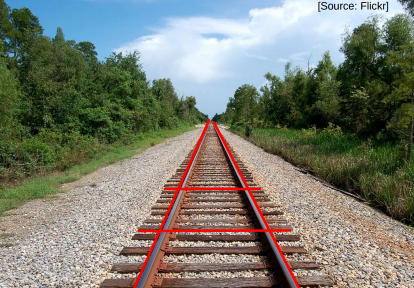
\includegraphics[height=4cm]{img/railway_tracks.png}
    \caption{Two properties of the pinhole-based projection; parallel lines meet, straight lines remain straight (project to straight lines).}
    \label{fig:my_label}
\end{figure}

\subsubsection{Definition}

% https://www.youtube.com/watch?v=MQdm0Z_gNcw
\marginnote{Upright style $\textbf{\textup{x}}$ will be used for H.C. vectors and italic $\textbf{\textit{x}}$ for Euclidean.}Homogeneous coordinates are useful for representing an object up to a scale. Mathematically, if $\textbf{\textup{x}}$ represents a point in the H.C. space, then $\lambda \textbf{\textup{x}}, \; \lambda \neq 0$ must represent the same point, i.e. $\textbf{x}$ and $\lambda\textbf{x}$ must be equivalent ($\sim$) in H.C. We denote equivalencies in H.C. with $\sim$, therefore $\bx \sim \lambda \bx$. A point in the H.C. space is defined only by its direction and not by its magnitude. The H.C. for 3D points are hence defined as follows.
\begin{definition}[Homogeneous Coordinates of a 3D vector]
% ref https://www.robots.ox.ac.uk/~dwm/Courses/AIMS/AIMS-L3.pdf
A Euclidean 3D point $\bx = (x,\, y,\, z)\t$ is represented in \emphasis{homogeneous coordinates} by ANY 4-vector $(x_1,x_2,x_3,x_4)\t$ such that:
\begin{equation}
    x = \frac{x_1}{x_4}, \quad y = \frac{x_2}{x_4}, \quad z = \frac{x_3}{x_4}, \quad \textup{in \quad H.C.:} \quad
    \textbf{\textup{x}} = (x_1, x_2, x_3, x_4)\t
    \label{eq:ec_to_hc}
\end{equation}
\end{definition}
$x_4$ can attain any value. For instance for $x_4=1$ the H.C. of $(x,y,z)$ are $(x,y,z,1)$. The following lemma is therefore straightforward.
\marginnote{Converting from E.C.to H.C. is NOT unique! Converting H.C. to E.C. is unique.}
\begin{lemma}
In H.C., $\begin{bmatrix}x_1 & x_2 & x_3 & x_4\end{bmatrix}\t$ and $\lambda \begin{bmatrix}x_1 & x_2 & x_3 & x_4\end{bmatrix}\t,\; \lambda \neq 0$  represent the same point, i.e.
\begin{equation}
    \textbf{\textup{x}} \sim \lambda \textbf{\textup{x}}, \quad \textbf{\textup{x}} = \begin{bmatrix}x_1 & x_2 & x_3 & x_4\end{bmatrix}\t, \quad \lambda \neq 0
\end{equation}
\label{lem:hc_equiv}
\end{lemma}
% ref https://cg.informatik.uni-freiburg.de/course_notes/graphics_02_transformations.pdf
For example, $(2,3,4,1) \sim (6,9,12,3) \sim (2,3,4)$, and $(4,8,12,2)\sim (2,4,6)$. 

\subsubsection{Converting between Euclidean and homogeneous coordinates}

From Lemma \ref{lem:hc_equiv}, it is clear that to convert a point $(x,y,z)$ from Euclidean to H.C. we simply add one more ordinate $w=1$ and obtain $(x,y,z,1)$. From now on black dot ($\bullet$) denotes H.C. and white ($\circ$) E.C.
\begin{equation}
\begin{bmatrix}
x_1 \\ x_2 \\ x_3    
\end{bmatrix}
\laplace
\begin{bmatrix}
x_1 \\ x_2 \\ x_3 \\ 1
\end{bmatrix}
\end{equation}
% ref https://www.robots.ox.ac.uk/~dwm/Courses/AIMS/AIMS-L3.pdf
Inversely, to ``dehomogenise'' a point $(x_1,\, x_2,\, x_3,\, x_4)\t, \; x_4 \neq 0$, we first divide its elements by $x_4$ such that the last element is $1$. We then discard the last element to obtain $(x_1/x_4,\, x_2/x_4,\,  x_3/x_4)$.
\begin{equation}
\begin{bmatrix}
    x_1 \\ x_2 \\ x_3 \\ x_4
\end{bmatrix}
\Laplace
\begin{bmatrix}
    x_1/x_4 \\ x_2/x_4 \\ x_3/x_4
\end{bmatrix}, \quad x_4 \neq 0
\end{equation}
\marginnote{$\bullet$ for H.C., $\circ$ for E.C.}For example, $(1,2,3,4)\t \sim (3,6,9,12)\t \sim (-2,-4,-6,-8)\ \Laplace \ (0.25, 0.5, 0.75)$ and they all represent the 3D point Also $(0,0,2) \sim (0,0,\pi)\ \Laplace \ (0,0)$.
\begin{exmp}
% ref http://users.telenet.be/jci/math/homog.htm
Calculate the midpoint between $\textbf{\textup{p}}_1=(5,7,8)$ and $\textbf{\textup{p}}_2 = (4,-6,1)$.
\end{exmp}
\begin{soln}
\marginnote{Distance ratios are not preserved in when converting between E.C. and H.C.}
We convert to E.C. to find the midpoint.
\begin{align*}
\textbf{\textup{p}}_1 = (5,7,8)\ \Laplace \ (5/8,7/8) := \textbf{\textit{p}}_1
,\\
\textbf{\textup{p}}_2 = (4,-6,1)\ \Laplace \ (4,-6) := \textbf{\textit{p}}_2
\end{align*}
The midpoint in E.C. is $(\textbf{\textit{p}}_1 + \textbf{\textit{p}}_2)/2 = (37/16,-41/16) \  \Laplace \ (37/16, -41/16, 1) \sim (37, -41, 16) $ 
\end{soln}
% ex: \textbf{https://web.stanford.edu/class/cs231a/course_notes/01-camera-models.pdf}


\subsubsection{Geometric interpretation of homogeneous points}

If we were to convert a 2D point in E.C $(x_1, y_1)$ to H.C., we would augment:
\[
\begin{bmatrix}
x_1 \\ x_2    
\end{bmatrix}
\laplace
\begin{bmatrix}
x_1 \\ x_2  \\ 1
\end{bmatrix}
\]
Therefore in a 3D plane, the point $(x_1,x_2,1)$ in H.C. can be geometrically determined by looking at the direction $(x_1, x_2)$ and at height $x_3=1$ from the origin. Of course, because $(x_1,x_2,1) \sim \lambda(x_1,x_2,1)$, point $(x_1,x_2,1)$ is also found at $(2x_1,2x_2,2)$, $(2.5x_1,2.5x_2,2.5)$, etc. but as a convention we will be taking $x_3=1$.

Projecting onto $x_3 = 1$ helps us also find the E.C. representation of the projected point -- if $x_3=1$, then the E.C. are simply $(x_1, x_2)$. Because the projected point is expressed as $(x/w, y/w, 1)$ (Fig. \ref{fig:hc_vis_in_R3}), if we plug in $x=0,\ y=0$, then we observe that the origin $O_2(0,0)$ in E.C. gets mapped to $O_3(0,0,1)$ in H.C.
\begin{figure}[H]
    % ref left: https://www-m10.ma.tum.de/foswiki/pub/Lehre/WS0809/GeometrieKalkueleWS0809/ch3.pdf, ref middle: https://w2.mat.ucsb.edu/594cm/2010/Week1/homog-coords.pdf, ref right: https://pages.mtu.edu/~shene/COURSES/cs3621/NOTES/geometry/homo-coor.html
    \centering
    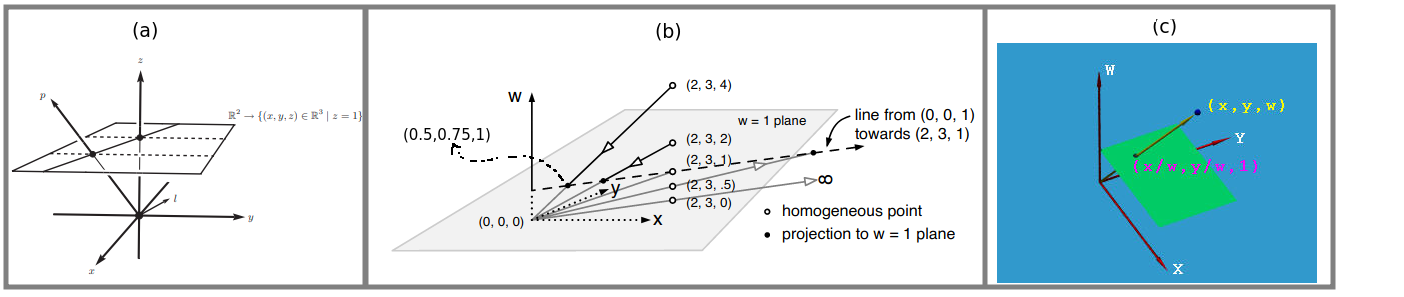
\includegraphics[width=1.08\linewidth]{img/hom_point_vis.png}
    \caption{(a): The set of homogeneous points $(x,y,z)$ in the $\setR^3$ space. (b): Numerical example of homogeneous points projected on $z=1$. (c): To project to $z=1$, we divide all ordinates by $w$.}
    \label{fig:hc_vis_in_R3}
\end{figure}


%fig: https://w2.mat.ucsb.edu/594cm/2010/Week1/homog-coords.pdf

\subsection{Mathematics of lines and points in 3D}

We have to describe the mathematics of lines in the projected space (2D) since this is what cameras use. As we will see, H.C. make it easier than Euclidean. Suppose we have a 2D point represented in E.C. as $\textit{\textit{x}} = (x,y)$. If this point lies on a line, then this line is defined by some $a_1,\, a_2,\, a_3$ such that: $a_1x + a_2y + a_3 = 0, \; a_1 \neq 0$ or $a_2\neq 0$. We can rewrite this equation for in H.C. if we convert $\textbf{\textit{x}} = (x,y) \; \laplace \;  \textbf{\textup{x}} = (x_1,x_2,x_3)$ by following \eqref{eq:ec_to_hc}:
\[
x = \frac{x_1}{x_3}, \quad y = \frac{x_2}{x_3}, \quad x_3\in \setR*
\]
% ref https://web.cs.iastate.edu/~cs577/handouts/homogeneous-coords.pdf
Then the line is written in H.C. as:
\begin{gather}
    a_1x + a_2y + a_3 = 0 \Rightarrow \nonumber \\
    a_1 \frac{x_1}{x_3} + a_2 \frac{x_2}{x_3} + a_3 = 0 \Rightarrow \nonumber \\
    a_1 x_1 + a_2 x_2 + a_3 x_3 = 0 \Rightarrow \nonumber \\
    \boldsymbol{\ell}\t \textbf{\textup{x}} = 0, \quad \boldsymbol{\ell} = (a_1,\, a_2,\, a_3)\t \nonumber
\end{gather}

\marginnote{$s\elll, \; s \in \setR^*$ and $\elll$ encode the same line.}
\begin{corollary}[line equation in H.C.]
If a 2D point  $(x,y)$ in E.C.  lies on a line parametrised by $(a_1,a_2,a_3)$, then in H.C. the line equation is described by a dot product:
\begin{equation}
    \boldsymbol{\ell}\t \textbf{\textup{x}}  = 0, \quad \boldsymbol{\ell}\t = (a_1,\, a_2,\, a_3)\t, \quad a_1,\, a_2 \neq 0
    \label{eq:line_hc}
\end{equation}
\end{corollary}
\eqref{eq:line_hc} allows us to concisely express the intersection of two lines and the line through two points.
\begin{corollary}[intersection of lines in H.C.]
Consider the two parametrised lines $\elll_1 = (a_1,a_2,a_3)\t$, $\elll_2 = (b_1,b_2,b_3)$ in H.C. Then they intersect at point $\textbf{p} = \elll_1 \times \elll_2$, where $\times$ denotes cross product.
\label{cor:inters_lines_hc}
\end{corollary}
\begin{proof}
Let $\textbf{p}$ be the point (in H.C.) where $\elll_1$ and $\elll_2$ intersect. Therefore $\textbf{p}$ satisfies the line equation \eqref{eq:line_hc} for both lines
\begin{align*}
    \textbf{p} \cdot \elll_1 = 0\\
    \textbf{p} \cdot \elll_2 = 0
\end{align*}
, where $\textbf{p} \cdot \elll_1 =\textbf{p} \t \elll_1$ is a dot product. We don't care about the magnitude of $\textbf{p}$, we only need such a vector that is perpendicular to both $\elll_1$ and $\elll_2$. Such a vector is by its definition the cross product $\elll_1\times \elll_2$, i.e.
\[
(\underbrace{\elll_1\times \elll_2}_{\textbf{p}})\cdot \elll_1 = (\underbrace{\elll_1\times \elll_2}_{\textbf{p}})\cdot \elll_2 = 0
\]
\begin{figure}[H]
    \centering
    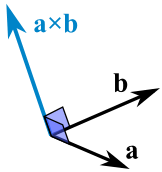
\includegraphics[height=2cm]{img/cross_product_vis.png}
    \caption{The cross product $\ba\times \bb$ is perpendicular to both $\ba$ and $\bb$.}
    \label{fig:my_label}
\end{figure}
\end{proof}

\begin{corollary}[line joining two points in H.C.]
If $\textbf{\textup{p}}_1, \, \textbf{\textup{p}}_2$ are two points in H.C., then the coefficients of the line joining them can be computed from $\elll = \textbf{\textup{p}}_1 \times \textbf{\textup{p}}_2$.
\label{cor:line_joining_pt_hc}
\end{corollary}
\begin{proof}
We want both $\textbf{p}_1$ and $\textbf{p}_2$ to lie on the same line, i.e. satisfy its equation:
\begin{align*}
    \textbf{p}_1 \cdot \elll = 0\\
    \textbf{p}_2 \cdot \elll = 0
\end{align*}
As shown the previous proof, to satisfy these two conditions we can choose $\elll = \textbf{p}_1\times \textbf{p}_2$.
\end{proof}
Note that Cor. \ref{cor:line_joining_pt_hc} is \textit{dual} to Cor. \ref{cor:inters_lines_hc}, in the sense that points and lines are swapped. This occurs because both points and lines are represented by 3D vectors. Fig. \ref{fig:duality_vis} visualises geometrically Cor. \ref{cor:line_joining_pt_hc} and Cor. \ref{cor:inters_lines_hc} in H.C.

\begin{figure}[H]
    % ref https://www.tugraz.at/fileadmin/user_upload/Institute/ICG/Documents/courses/robotvision/2019/RV_ProjectiveGeometry.pdf
    \centering
    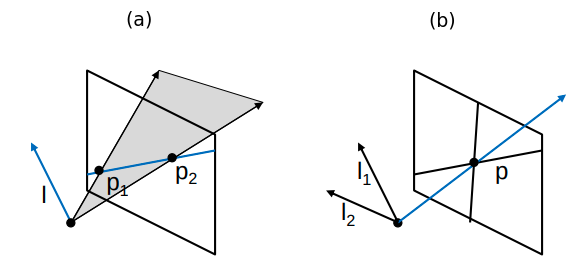
\includegraphics[height=3.75cm]{img/duality_vis.png}
    \caption{(a): The vector $\textbf{l}$ with the coefficients of the line joining $\textbf{p}_1, \textbf{p}_2$ is perpendicular to both $\textbf{p}_1$ and $\textbf{p}_2$ vectors, therefore perpendicular to the plane they span. (b): The same principle holds for a point $\textbf{p}$ which at the intersection of lines $\textbf{l}_1, \textbf{l}_2$.}
    \label{fig:duality_vis}
\end{figure}

% ref https://web.cs.iastate.edu/~cs577/handouts/homogeneous-coords.pdf, https://pages.mtu.edu/~shene/COURSES/cs3621/NOTES/geometry/homo-coor.html
Points at infinity $(\pm \infty, \pm \infty)$ can be represented in H.C. by finite quantities. To verify that, consider all points starting from $\textbf{\textit{r}}_0 = (x_0,y_0)$ with direction $\textbf{v} = (a,b)$. Then, points given by $\textbf{\textit{r}} = \textbf{\textit{r}}_0 + t\textbf{v},\; t\in\setR$ lie along the same straight line. Each scalar component of $\textbf{\textit{r}}$ is given by:
\begin{equation*}
    x = x_0 + ta, \quad y = y_0 + tb \tag{1}
    \label{eq:param_3d_line}
\end{equation*}
\eqref{eq:param_3d_line} is the parametric line equation of the 2D line where points $\textbf{\textit{r}} = (x,y,z) = (x_0 + ta, y_0 + tb, z_0 + tc)$ lie. In H.C., points of $\textbf{\textit{r}}$ are given by $\textbf{r} = (x_0 + ta, y_0 + tb, 1)$. Because $\textbf{r} = \textbf{r}/t$ in H.C., they are also given by:
\[
\textbf{r} = (\frac{x_0}{t} + a, \frac{y_0}{t} + b, \frac{1}{t}) 
\label{eq:line_2d_hc}
\tag{2}
\]
The E.C. points $(x_0 + ta, y_0 + tb, z_0 + tc)$ approach infinity as $t\rightarrow \infty$. If we plug in $t\rightarrow \infty$ in \eqref{eq:line_2d_hc}, it turns out the points in infinity in H.C. are given by:
\[
\textbf{r} = (a, b , 0) 
\]
 Moving in the directions of $(a,b)$ and $(-a, -b)$ will end up at the same infinity point represented by $(a,b,0)$ as well as $(-a, -b, 0)$. For instance, the points at infinity in the direction vector $\textbf{v}=(-3,2)$ are given by $(-3,2,0)$ in H.C. and all lie on the line $y=-2/3x$.
 \begin{figure}[H]
    % ref https://www.math.ucla.edu/~baker/149.1.02w/handouts/m_hcoords.pdf
     \centering
     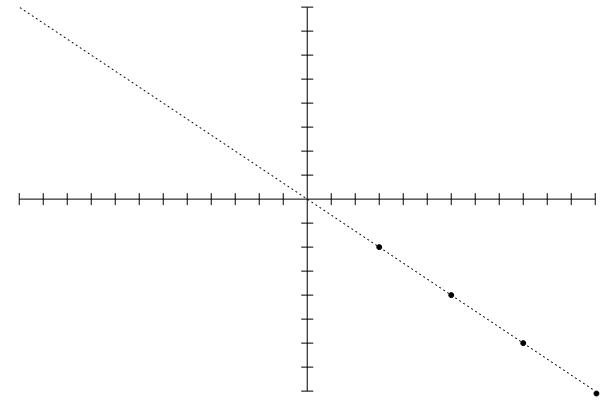
\includegraphics[height=3.5cm]{img/points_inf_graph.png}
     \caption{Points at infinity along the direction $(-3,2)$}
 \end{figure}
\begin{corollary}[point at infinity in H.C.]
In H.C., points of the form $(a, b, 0)$ represent a point that tends to infinity in E.C. in the direction of $\textbf{v} = (a,b)$. They're also known as \emphasis{ideal points}.
\end{corollary}
% ref http://lear.inrialpes.fr/people/triggs/pubs/isprs96/node7.html
Ideal points all lie along the same line $\elll$. If $\elll = (l_1,l_2,l_3)$ in H.C., then all ideal points $(a,b,0)$ must satisfy
\begin{align*}
    \begin{bmatrix}l_1 & l_2 & l_3\end{bmatrix}\t \begin{bmatrix}a & b & 0\end{bmatrix} = 0 \Rightarrow
    a = 0, \quad b = 0,\quad c \in \setR
\end{align*}
Therefore all ideal points lie along the line with coefficients $(0,0,c) \sim (0,0,1)$ in H.C. To summarise:
\begin{corollary}[line at infinity]
All ideal points lie along the line $\elll_{\infty} = (0,0,1)$ in H.C. This is known as \emphasis{ideal line}.
\end{corollary}
Ideal points are important because that's where lines that are parallel in E.C. meet. To verify that, consider the equations of two parallel lines:
\begin{align*}
\left\{ 
\begin{matrix}
a_1x + b_1y + c_1 = 0\\
a_1x + b_1y + c_2 = 0 \\
\end{matrix}, \quad c_1 \neq c_2
\right.
\label{eq:2parallel_lines_ec}
\end{align*}
Therefore in H.C., they can be described by $\elll_1 = (a_1, b_1, c_1)$, $\elll_2 = (a_1, b_1, c_2)$. From Cor. \ref{cor:inters_lines_hc}, we know that they intersect at:
\begin{align*}
\textbf{p} &= \elll_1 \times \elll_2 \\  
&= \left|
\begin{matrix}
\textbf{i} & \textbf{j} & \textbf{k} \\
a_1 & b_1 & c_1 \\
a_1 & b_1 & c_2
\end{matrix}
\right| = \textbf{i} (b_1c_2 - b_1c_1) + \textbf{j} (a_1c_2 - a_1c1) + \textbf{k}\cdot 0 \\
&= (b_1c_2 - b_1c_1, a_1c_2 - a_1c1, 0)
\end{align*}
$(b_1c_2 - b_1c_1, a_1c_2 - a_1c1, 0)$ is an ideal point. To summarise:

\begin{corollary}[intersection of parallel lines in H.C.]
Two parallel lines in H.C., $\elll_1 = (a, b, c)$ and $\elll_2 = (a, b, d), \quad c \neq d$ intersect at an ideal point $\textbf{\textup{p}}$ (point at infinity) given by:
\begin{equation}
    \textbf{\textup{p}} = (b(d-c), a(d-c), 0)
\end{equation}
\end{corollary}

In conclusion, very concept in projective geometry has its dual. If we start with a certain statement, e.g. ``The \textcolor{magenta}{\underline{line}} \textcolor{magenta}{\underline{joining}} \textcolor{magenta}{\underline{points}} $\textbf{p}_1$, $\textbf{p}_2$ is given by $\elll = \textbf{p}_1\times \textbf{p}_2$''  and take the dual of each concept, we end up with ``The \textcolor{magenta}{\underline{point}} of \textcolor{magenta}{\underline{intersection}} of  \textcolor{magenta}{\underline{lines}} $\textbf{l}_1$, $\textbf{l}_2$ is given by $\textbf{p} = \elll_1\times \elll_2$''. For completeness, the duality table is given below.
\begin{table}[h!]
\centering
 \begin{tabular}{c c} 
 \hline
 Original & Dual\\ [0.5ex] 
 \hline
 point & line \\
 join & intersect \\
 $\textbf{p}$ & $\elll$ \\
 [1ex] 
 \hline
 \end{tabular}
\end{table}

\subsubsection{Geometric interpretation of conversions between E.C. and H.C.} 
% https://medium.com/@daniel.j.lenton/part-i-projective-geometry-in-2d-b1ca26d5fa2a and TODOs

So far 2D E.C. points were described as infinite rays in the 3D Euclidean space. In this section H.C. points are described in an alternative geometrical fashion -- as straight 2D line segments. The most important thing to remember to interpret H.C. coordinates this way is that an infinite line through the origin is normal to a (3D) plane through the origin. In this section, the following are described in Euclidean space:
\begin{enumerate}
    \item H.C. points,
    \item a line intersection in H.C.,
    \item and the points of the line joining two H.C. points
\end{enumerate}

Below each case is derived geometrically.
\begin{enumerate}
    \item (\textbf{H.C. point in E.C. space}) We already know that a H.C. point $(\ell_1, \ell_2, \ell_3)$ lies anywhere along the straight line from the origin to $\lambda(\ell_1, \ell_2, \ell_3), \; \lambda \in \setR$. The line defined by the direction of $(\ell_1, \ell_2, \ell_3)$ is normal to a plane through the origin that is normal to it, i.e. to plane $\ell_1x_1 + \ell_2x_3 + \ell_3x_3 = 0$. Also, to find the Euclidean equivalent of a H.C. point, we set $x_3=1$. Ultimately, the Euclidean equivalent of the H.C. point $(\ell_1, \ell_2, \ell_3)$ is determined by the intersection of the following two planes:
    \[
    \ell_1x_1 + \ell_2x_2 + \ell_3x_3 = 0 \quad \cap \quad   x_3 - 1 = 0
    \]
    Therefore the 2D line equation that describes point $(\ell_1,\ell_2,\ell_3)$ is:
    \[
        \ell_1x_1 + \ell_2x_2 + \ell_3 = 0 
    \]
    All this is visualised in Fig. \ref{fig:geo_plane_origin} and Fig. \ref{fig:geo_point_in_line}.
\begin{figure}[H]
    \centering
    \begin{minipage}{.4\textwidth}
      \centering
      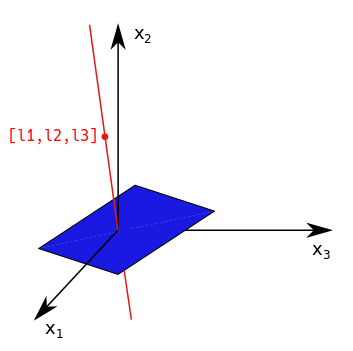
\includegraphics[width=0.7\linewidth]{img/geo_plane_origin.png}
      \captionof{figure}{The plane $\ell_1x_1 + \ell_2x_2 + \ell_3x_3 = 0$}
      \label{fig:geo_plane_origin}
    \end{minipage}%
    \begin{minipage}{.5\textwidth}
      \centering
      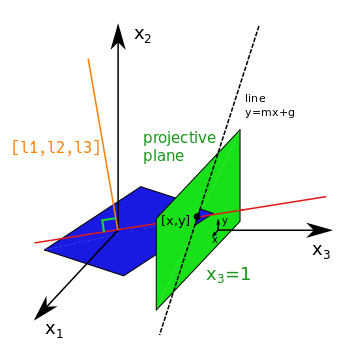
\includegraphics[width=.7\linewidth]{img/geo_point_in_line.png}
      \captionof{figure}{The intersection of plane$\ell_1x_1 + \ell_2x_2 + \ell_3x_3 = 0$ with $x_3=1$ describes H.C. point $(\ell_1, \ell_2, \ell_3)$ as a 2D straight line.}
      \label{fig:geo_point_in_line}
    \end{minipage}
\end{figure}

    \item (\textbf{line intersection in H.C.}) We now know that a line along point $\elll = (\ell_1, \ell_2, \ell_3)$ in H.C. can be represented as the intersection of planes $\elll\t \bx=0$, $x_3 = 1$ in the 3D space. Also the intersection of two E.C. points $\elll = (\ell_1, \ell_2, \ell_3)$, $\textbf{m} = (m_1, m_2, m_3)$ can be described as an infinite ray spanned by the cross product $\elll \times \textbf{m}$ (Cor. \ref{cor:line_joining_pt_hc}). Finally, to convert ray $\elll \times \textbf{m}$ to its E.C. equivalent, we project it onto plane $x_3=1$
    
    This is visualised in the figure below, where the red and blue planes are given, the orange ray describes their cross product, and the intersection of the orange ray with plane $x_3=1$ (which is a straight line) describes the intersection of the two lines defined by $\elll = (\ell_1, \ell_2, \ell_3)$ and  $\textbf{m} = (m_1, m_2, m_3)$ respectively. Note that the orange ray is NOT necessarily along the axis $x_3$, although the figure is misleading.
    
    \begin{figure}[H]
        \centering
        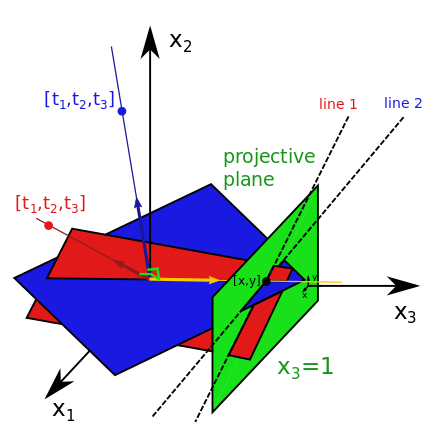
\includegraphics[height=5cm]{img/geo_intersection_of_lines.png}
        \caption{Intersection of H.C. lines $\elll = (\ell_1, \ell_2, \ell_3)$ and  $\textbf{m} = (m_1, m_2, m_3)$ described as a 2D line.}
    \end{figure}
    
    \item (\textbf{Line joining two H.C. points}) It is known from Cor. \ref{cor:line_joining_pt_hc} that if two H.C. points $\textbf{p}_1$, $\textbf{p}_2$ are given , then the coefficients of the line through them in H.C. are given by the cross product $\elll = \textbf{p}_1 \times \textbf{p}_2$. This cross product is once again a vector normal to the plane $\elll_1x_1 + \elll_2x_2 + \elll_3x_3 = 0$. To unproject the plane $\elll\t\bx=0$ in 2D, we project it onto $x_3=1$. The line projected onto $x_3=1$ describes the line through $\textbf{p}_1$ and $\textbf{p}_2$ in 2D.
    \begin{figure}[H]
        \centering
        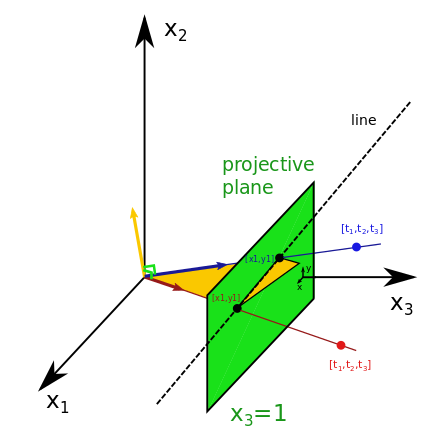
\includegraphics[height=5cm]{img/geo_line_two_points.png}
        \caption{The intersection of the plane $(\textbf{p}_1\textbf{p}_2)\t\bx=0$ with $x_3=1$ describes the line through H.C. points $\textbf{p}_1$ and $\textbf{p}_2$.}
    \end{figure}


\end{enumerate}




\subsection{The cross ratio}
% http://cs.rkmvu.ac.in/~sghosh/public_html/bhu_igga/tute.pdf
%http://www.ipb.uni-bonn.de/html/teaching/3dcs-ge-2020/stachniss/2020-3dcs-02-homogeneous-coords-4.pdf
%https://beckassets.blob.core.windows.net/product/readingsample/6715665/9783642172854_excerpt_001.pdf
% https://teaching.csse.uwa.edu.au/units/CITS4402/lectures/Lecture09-ProjectiveGeometry.pdf
% http://users.umiacs.umd.edu/~ramani/cmsc828d/ProjectiveGeometry.pdf
% https://teaching.csse.uwa.edu.au/units/CITS4402/lectures/Lecture09-ProjectiveGeometry.pdf
% https://filebox.ece.vt.edu/~jbhuang/teaching/ece5554-4554/fa17/lectures/Lecture_12_CalibrationAndMetrology.pdf
% https://mi.eng.cam.ac.uk/~cipolla/lectures/4F12/Examples/4F12-examples-2.pdf


%=-=-=-=-=-=-=-=-=-=-=-=-=-=-=-=-=-=-=-=-=-=-=-=-=-=-=-=-=-=-=-=-=-=-=-=-=-=-=-=-
% References
%=-=-=-=-=-=-=-=-=-=-=-=-=-=-=-=-=-=-=-=-=-=-=-=-=-=-=-=-=-=-=-=-=-=-=-=-=-=-=-=-
\newpage
\printbibliography



%=-=-=-=-=-=-=-=-=-=-=-=-=-=-=-=-=-=-=-=-=-=-=-=-=-=-=-=-=-=-=-=-=-=-=-=-=-=-=-=-
% Appendices
%=-=-=-=-=-=-=-=-=-=-=-=-=-=-=-=-=-=-=-=-=-=-=-=-=-=-=-=-=-=-=-=-=-=-=-=-=-=-=-=-
\newpage
\appendix

\section{Appendices}

% ------------------------ New appendix ------------------------ %
\newpage
\subsection{Pinhole camera model derivation}
\label{app:pinhole_model_deriv}

%\lstinputlisting[language=python,caption={A code listing (\detokenize{src/foo_bar.py)}.}, label=src:mylabel]{src/foo_bar.py}
   Consider the case of a \textit{pinhole camera}, which consists of a box which a tiny aperture on the front plane and a film which captures the energy (colour) of the light on the real plane (Fig. \ref{fig:pinhole_model}). We assume that all light rays entering the camera meet at the aperture (centre of projection). The horizontal distance between the aperture and the film is called \emphasis{focal length} $f$.
    \begin{figure}[H]
        \centering
        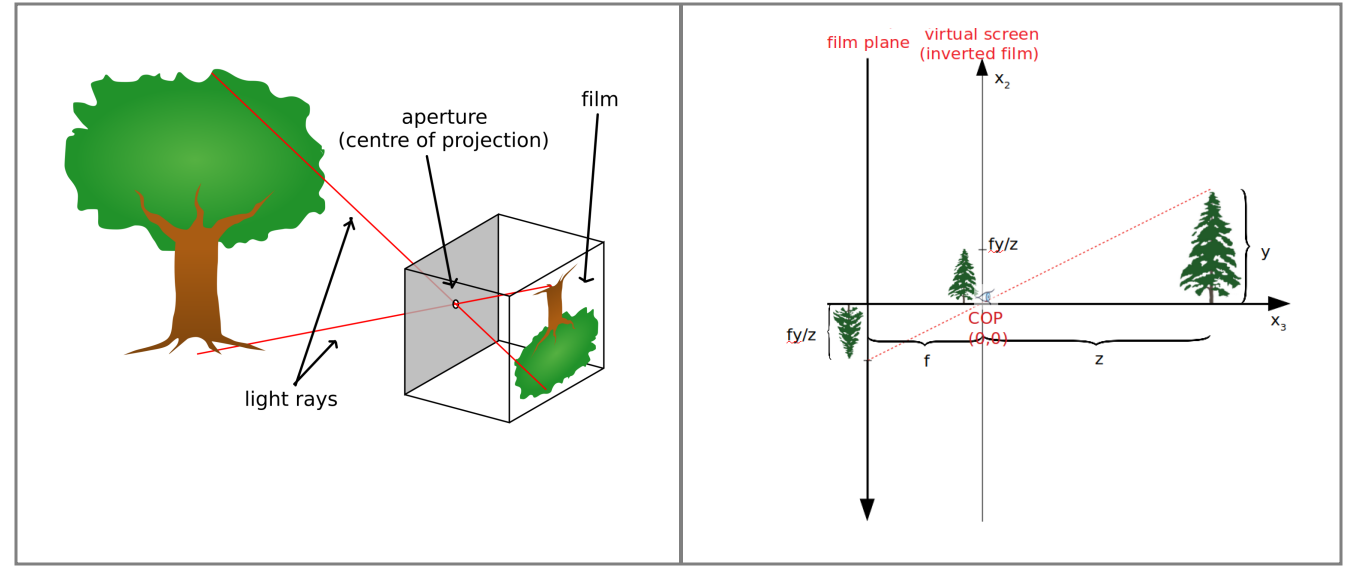
\includegraphics[height=6cm]{img/pinhole_model.png}
        \caption{Left: Pinhole camera schematic in 3D. Right: Pinhole camera model of a tree in the $y$ dimension.}
        \label{fig:pinhole_model}
    \end{figure}

    From the similar triangles in front and behind the screen in Fig. \ref{fig:pinhole_model}, we obtain for the project $y\prime$ of the object:
    \marginnote{The position $(x',y')$ on the screen is measured in distance units -- not pixels.}
    \[
        \frac{y}{z} = \frac{y\prime}{f} \Rightarrow y\prime = f\frac{y}{z}
    \]
    Similarly for the projected $x\prime$ (not shown in Fig. \ref{fig:pinhole_model}) we obtain:
    \[
        x\prime = f\frac{x}{z}
    \]
    To reiterate, pinhole camera performs the following linear mapping in Caertesian coordinates:
    \[
        \begin{bmatrix}
            x \\ y \\ z
        \end{bmatrix} \mapsto
        \begin{bmatrix}
            \frac{fx}{z} \\
            \frac{fy}{z} 
        \end{bmatrix}, \qquad 
        \begin{bmatrix}
            \frac{fx}{z} \\
            \frac{fy}{z} 
        \end{bmatrix} = 
         \frac{1}{z}\begin{bmatrix}
            f & 0 & 0 \\
            0 & f & 0 \\
            0 & 0 & 1
        \end{bmatrix}
        \begin{bmatrix}
            x \\ y \\ z
        \end{bmatrix}
        \]


\end{document}